% !TEX root = ../main.tex
% File: chapters_part1/chap6_3.tex
% Nội dung cho Chương 6, Phần 3

\section{Mô hình Đa phương thức (Multimodal Models)}
\label{sec:multimodal_models}

Con người trải nghiệm thế giới thông qua nhiều giác quan cùng một lúc: chúng ta nhìn thấy một hình ảnh, nghe một âm thanh, và đọc một đoạn văn bản mô tả về nó. Các mô hình mà chúng ta đã thảo luận cho đến nay chủ yếu là đơn phương thức (unimodal) - chúng chỉ xử lý văn bản. Để AI thực sự tiến gần hơn đến trí thông minh của con người, chúng cần có khả năng hiểu và lý luận trên nhiều loại dữ liệu khác nhau một cách đồng thời. Đây chính là mục tiêu của các \textbf{Mô hình Đa phương thức (Multimodal Models)}.

Lĩnh vực này đã có những bước nhảy vọt phi thường, đặc biệt là trong việc kết hợp hai phương thức quan trọng nhất: \textbf{Ngôn ngữ (Language)} và \textbf{Thị giác (Vision)}. Phần này sẽ đi sâu vào các kiến trúc nền tảng đã tạo nên cuộc cách mạng này.

\subsection{Nền tảng: Xây dựng cầu nối giữa Ảnh và Chữ}
\label{ssec:multimodal_foundations}

Để một mô hình có thể hiểu cả ảnh và chữ, nó cần một "ngôn ngữ chung" - một không gian biểu diễn nơi cả ảnh và chữ đều có thể được ánh xạ vào và so sánh với nhau. Hai đột phá nền tảng đã tạo ra cây cầu này là Vision Transformer (ViT) và Contrastive Learning (CLIP).

\subsubsection{Vision Transformer (ViT): "Đọc" ảnh như đọc một câu}
\paragraph{Vấn đề với CNN}
Các mạng CNN (đã học ở mục \ref{sec:cnn_for_nlp}) xử lý ảnh bằng cách trượt các bộ lọc nhỏ, xây dựng các đặc trưng từ cục bộ (cạnh, góc) đến toàn cục (mắt, mũi, khuôn mặt). Cách tiếp cận này rất hiệu quả nhưng lại có một sự khác biệt về kiến trúc so với Transformer đang thống trị NLP.

\paragraph{Giải pháp của ViT: Biến ảnh thành một chuỗi các "từ"}
Vision Transformer (Dosovitskiy et al., 2020) đã đưa ra một ý tưởng cấp tiến:
\begin{tcolorbox}[
    title=Trực giác của Vision Transformer,
    colback=blue!5!white, colframe=blue!75!black, fonttitle=\bfseries
]
"Điều gì sẽ xảy ra nếu chúng ta coi một bức ảnh không phải là một lưới pixel, mà là một \textbf{chuỗi các mảnh vá (sequence of patches)}? Nếu vậy, chúng ta có thể đưa chuỗi các mảnh vá này vào một kiến trúc Transformer tiêu chuẩn, giống hệt như cách chúng ta xử lý một chuỗi các từ."
\end{tcolorbox}

\paragraph{Cơ chế hoạt động}
\begin{enumerate}
    \item \textbf{Phân mảnh Ảnh (Image Patching):} Một bức ảnh đầu vào (ví dụ: $224 \times 224$ pixel) được chia thành một lưới các mảnh vá không chồng chéo có kích thước cố định (ví dụ: $16 \times 16$ pixel). Điều này tạo ra một chuỗi gồm $(224/16)^2 = 14 \times 14 = 196$ mảnh vá.
    \item \textbf{Nhúng Mảnh vá (Patch Embedding):} Mỗi mảnh vá được "làm phẳng" (flatten) thành một vector dài và sau đó được chiếu qua một lớp tuyến tính để tạo ra một "patch embedding" có số chiều phù hợp với Transformer (ví dụ: 768 chiều).
    \item \textbf{Thêm Token Phân loại và Mã hóa Vị trí:} Tương tự như BERT, một token `[CLS]` có thể học được sẽ được chèn vào đầu chuỗi. Sau đó, các vector mã hóa vị trí (positional encodings) được cộng vào mỗi patch embedding để cung cấp thông tin về vị trí tương đối của các mảnh vá.
    \item \textbf{Đưa vào Transformer Encoder:} Chuỗi các patch embedding này giờ đây được xử lý bởi một chuỗi các khối Transformer Encoder tiêu chuẩn. Cơ chế Self-Attention sẽ cho phép mỗi mảnh vá "chú ý" đến tất cả các mảnh vá khác để học các mối quan hệ không gian.
\end{enumerate}

\begin{center}
    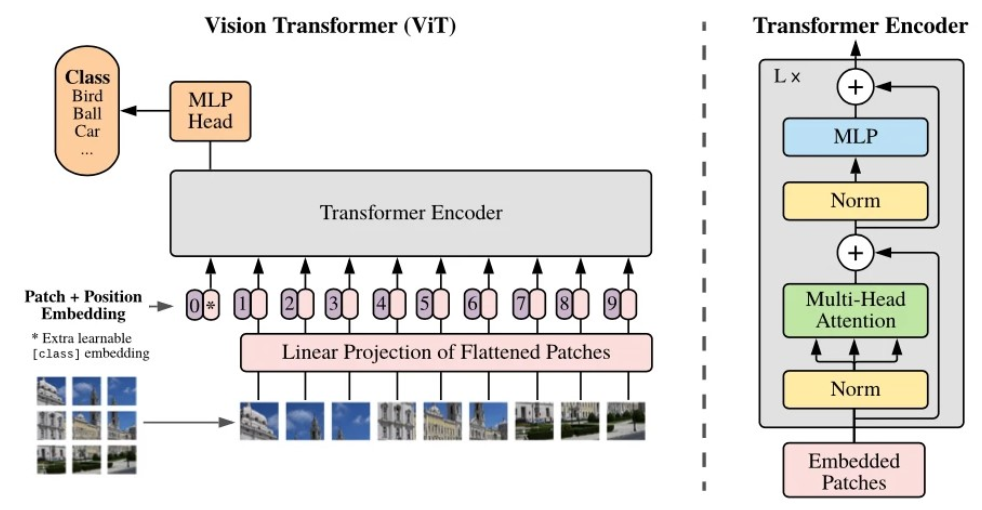
\includegraphics[width=1.0\textwidth]{vision_transformer_vit.png}
    \captionof{figure}{Kiến trúc của Vision Transformer (ViT). Ảnh được chia thành các mảnh vá, mỗi mảnh được nhúng và xử lý như một "token" trong một chuỗi bởi một Transformer Encoder tiêu chuẩn.}
    \label{fig:vision_transformer_vit}
\end{center}

ViT đã chứng minh rằng một kiến trúc dựa hoàn toàn trên Transformer có thể đạt được hiệu năng state-of-the-art trong các tác vụ thị giác, tạo ra một sự thống nhất về mặt kiến trúc giữa NLP và CV. Nó cung cấp một cách mạnh mẽ để có được các \textbf{bộ mã hóa hình ảnh (Image Encoders)} tạo ra các biểu diễn giàu ngữ cảnh cho ảnh.

\subsubsection{CLIP: Học sự tương đồng giữa Ảnh và Chữ bằng Contrastive Learning}
\paragraph{Vấn đề}
Chúng ta đã có Image Encoder (ViT) và Text Encoder (Transformer). Làm thế nào để chúng "nói chuyện" với nhau? Làm thế nào để mô hình biết rằng bức ảnh một chú chó và câu "a photo of a dog" là cùng một khái niệm?

\paragraph{Giải pháp của CLIP (Contrastive Language-Image Pre-training)}
CLIP (Radford et al., 2021) từ OpenAI đã giải quyết vấn đề này bằng một phương pháp huấn luyện quy mô lớn dựa trên \textbf{Học Tương phản (Contrastive Learning)}, một ý tưởng tương tự như Mạng Siamese (mục \ref{sec:siamese_networks}).

\paragraph{Cơ chế hoạt động}
\begin{enumerate}
    \item \textbf{Kiến trúc:} CLIP bao gồm hai bộ mã hóa riêng biệt:
        \begin{itemize}
            \item Một \textbf{Image Encoder} (ví dụ: ViT).
            \item Một \textbf{Text Encoder} (ví dụ: một Transformer).
        \end{itemize}
    \item \textbf{Dữ liệu Huấn luyện:} Một bộ dữ liệu khổng lồ gồm 400 triệu cặp \textbf{(ảnh, văn bản mô tả)} được thu thập từ Internet.
    \item \textbf{Mục tiêu Huấn luyện:} Huấn luyện cả hai bộ mã hóa từ đầu để chúng ánh xạ các cặp (ảnh, văn bản) tương ứng vào \textbf{cùng một vị trí} trong một không gian embedding đa phương thức chung.
    \item \textbf{Quy trình trong một batch:}
        \begin{enumerate}
            \item Lấy một batch gồm $N$ cặp (ảnh, văn bản).
            \item Đưa $N$ ảnh qua Image Encoder để có được $N$ vector ảnh ($I_1, \dots, I_N$).
            \item Đưa $N$ văn bản qua Text Encoder để có được $N$ vector văn bản ($T_1, \dots, T_N$).
            \item Tính toán độ tương đồng cosine giữa \textbf{tất cả} các cặp vector ảnh và văn bản có thể có, tạo ra một ma trận tương đồng $N \times N$.
            \item \textbf{Hàm mất mát tương phản:} Mục tiêu là làm cho độ tương đồng của các cặp \textbf{khớp đúng} (ví dụ: $I_i$ và $T_i$) trên đường chéo chính của ma trận là cao nhất, và độ tương đồng của tất cả các cặp \textbf{không khớp} ($I_i$ và $T_j$ với $i \neq j$) là thấp nhất.
        \end{enumerate}
\end{enumerate}

\begin{center}
    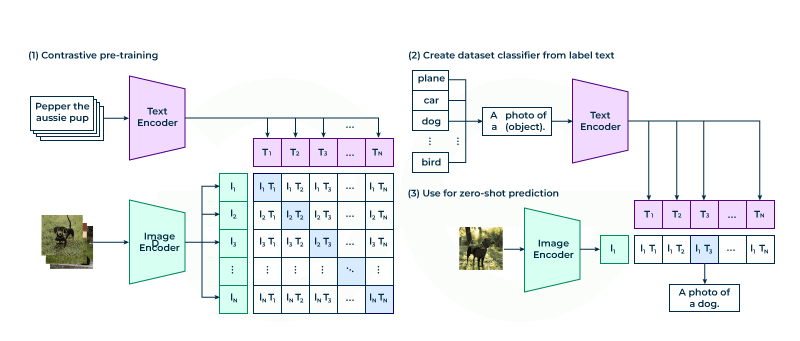
\includegraphics[width=1.0\textwidth]{clip_contrastive_learning.png}
    \captionof{figure}{Quy trình huấn luyện của CLIP. Mô hình học cách tối đa hóa độ tương đồng của các cặp (ảnh, văn bản) chính xác trên đường chéo chính và tối thiểu hóa độ tương đồng của các cặp không chính xác.}
    \label{fig:clip_contrastive_learning}
\end{center}

Sau khi huấn luyện, CLIP có khả năng zero-shot đáng kinh ngạc trong việc phân loại ảnh. Ví dụ, để phân loại một ảnh, bạn chỉ cần nhúng ảnh đó và so sánh độ tương đồng của nó với các vector văn bản được tạo từ các prompt như "a photo of a dog", "a photo of a cat",... và chọn prompt có độ tương đồng cao nhất.

Quan trọng hơn, CLIP đã tạo ra một \textbf{không gian embedding đa phương thức được căn chỉnh (aligned multimodal embedding space)} mạnh mẽ, là nền tảng cho các mô hình thế hệ tiếp theo.

\subsection{Ví dụ Kiến trúc: Kết hợp LLM với Thị giác}
\label{ssec:multimodal_architectures_examples}
Với các khối xây dựng là Image Encoder và không gian đa phương thức được căn chỉnh, các nhà nghiên cứu đã tạo ra các Mô hình Ngôn ngữ Lớn Đa phương thức (Multimodal Large Language Models - MLLMs).

\subsubsection{Flamingo: Thêm Cross-Attention vào một LLM đã đóng băng}
\begin{itemize}
    \item \textbf{Kiến trúc (Alayrac et al., 2022):} Flamingo giữ một LLM văn bản (ví dụ: Chinchilla) và một Vision Encoder (ví dụ: ViT) đã được huấn luyện trước và \textbf{đóng băng (frozen)} chúng.
    \item \textbf{Cơ chế kết nối:} Nó chèn các lớp \textbf{Cross-Attention} đặc biệt vào giữa các lớp của LLM.
    \item \textbf{Dòng chảy dữ liệu:} Khi xử lý văn bản, các token văn bản sẽ đi qua các lớp Transformer của LLM như bình thường. Tại các lớp Cross-Attention, các token văn bản này sẽ đóng vai trò là \textbf{Query}, trong khi các đặc trưng hình ảnh từ Vision Encoder sẽ đóng vai trò là \textbf{Key} và \textbf{Value}. Điều này cho phép các token văn bản "nhìn" vào hình ảnh và rút ra các thông tin thị giác liên quan khi cần thiết.
    \item \textbf{Lợi ích:} Rất hiệu quả về mặt tham số vì chỉ cần huấn luyện các lớp Cross-Attention mới.
\end{itemize}

\subsubsection{LLaVA: Ánh xạ Trực tiếp vào Không gian Từ của LLM}
LLaVA (Large Language and Vision Assistant - Liu et al., 2023) đưa ra một cách tiếp cận đơn giản hơn nhưng lại cực kỳ hiệu quả.
\begin{itemize}
    \item \textbf{Kiến trúc:} Sử dụng một Vision Encoder (cụ thể là ViT từ CLIP) và một LLM (cụ thể là Vicuna, một phiên bản của Llama).
    \item \textbf{Cơ chế kết nối:}
        \begin{enumerate}
            \item Ảnh được đưa qua Vision Encoder để tạo ra một chuỗi các patch embedding.
            \item Một \textbf{lớp chiếu tuyến tính (projection layer)} nhỏ duy nhất được huấn luyện để \textbf{ánh xạ (map)} các patch embedding này vào cùng một không gian với các word embedding của LLM.
            \item Các patch embedding đã được chiếu này sau đó được coi như các "từ" đặc biệt và được \textbf{chèn trực tiếp} vào chuỗi văn bản đầu vào của LLM.
        \end{enumerate}
    \item \textbf{Quá trình huấn luyện 2 giai đoạn:}
        \begin{enumerate}
            \item \textbf{Giai đoạn 1 (Căn chỉnh đặc trưng):} Đóng băng cả Vision Encoder và LLM, chỉ huấn luyện lớp chiếu tuyến tính trên một bộ dữ liệu lớn gồm các cặp (ảnh, mô tả). Giai đoạn này dạy cho lớp chiếu cách "dịch" đặc trưng ảnh thành "ngôn ngữ" mà LLM có thể hiểu.
            \item \textbf{Giai đoạn 2 (Tinh chỉnh End-to-End):} Mở đóng băng các trọng số của LLM và fine-tune toàn bộ mô hình (hoặc chỉ lớp chiếu và LLM) trên một bộ dữ liệu nhỏ hơn, chất lượng cao hơn gồm các chỉ dẫn đa phương thức phức tạp (ví dụ: các cuộc trò chuyện về hình ảnh).
        \end{enumerate}
    \item \textbf{Lợi ích:} Kiến trúc cực kỳ đơn giản, dễ triển khai và tận dụng được sức mạnh của các LLM và Vision Encoder đã có sẵn. LLaVA đã trở thành một trong những kiến trúc nền tảng cho các MLLM mã nguồn mở.
\end{itemize}

Sự kết hợp giữa Ngôn ngữ và Thị giác đang mở ra một kỷ nguyên mới của AI, nơi các mô hình có thể tương tác với thế giới một cách phong phú và tự nhiên hơn rất nhiều.

\subsection{Sinh Đa phương thức (Multimodal Generation)}
\label{ssec:multimodal_generation}

Nếu các mô hình ở mục trước tập trung vào việc \textit{hiểu} đầu vào đa phương thức (ví dụ, mô tả một bức ảnh bằng văn bản), thì một trong những bước đột phá ngoạn mục nhất của AI hiện đại là khả năng \textit{sinh} ra một phương thức từ một phương thức khác. Nổi bật nhất trong số đó là các tác vụ sinh từ văn bản, biến những mô tả trừu tượng thành các sản phẩm thị giác cụ thể.

\subsubsection{Sinh Ảnh từ Văn bản (Text-to-Image)}
Đây là lĩnh vực đã tạo ra một cuộc cách mạng trong ngành công nghiệp sáng tạo, cho phép bất kỳ ai cũng có thể tạo ra các tác phẩm nghệ thuật kỹ thuật số chỉ bằng ngôn ngữ.
\begin{itemize}
    \item \textbf{Bài toán:} Cho một câu mô tả bằng văn bản (prompt), ví dụ "một phi hành gia đang cưỡi ngựa trên sao Hỏa theo phong cách siêu thực", mô hình phải tạo ra một bức ảnh hoàn toàn mới khớp với mô tả đó.
    \item \textbf{Kiến trúc cốt lõi: Mô hình Khuếch tán (Diffusion Models)} Các mô hình thành công nhất hiện nay như DALL-E 2, Midjourney, và Stable Diffusion thường dựa trên kiến trúc này.
        \begin{enumerate}
            \item \textbf{Mã hóa Văn bản:} Prompt được đưa qua một bộ mã hóa văn bản mạnh mẽ (thường là một phần của mô hình CLIP) để tạo ra một vector embedding giàu ngữ nghĩa.
            \item \textbf{Quá trình Khuếch tán Ngược có Điều kiện:} Mô hình bắt đầu với một bức ảnh chỉ toàn nhiễu ngẫu nhiên (random noise). Sau đó, trong một chuỗi nhiều bước, một mạng nơ-ron (thường là U-Net) sẽ dần dần \textbf{khử nhiễu (denoise)} cho bức ảnh. Ở mỗi bước, quá trình khử nhiễu này được \textit{dẫn dắt} (conditioned) bởi vector embedding của văn bản. Quá trình này dần dần làm hiện ra một hình ảnh mạch lạc và khớp với prompt.
        \end{enumerate}
\end{itemize}
\begin{center}
    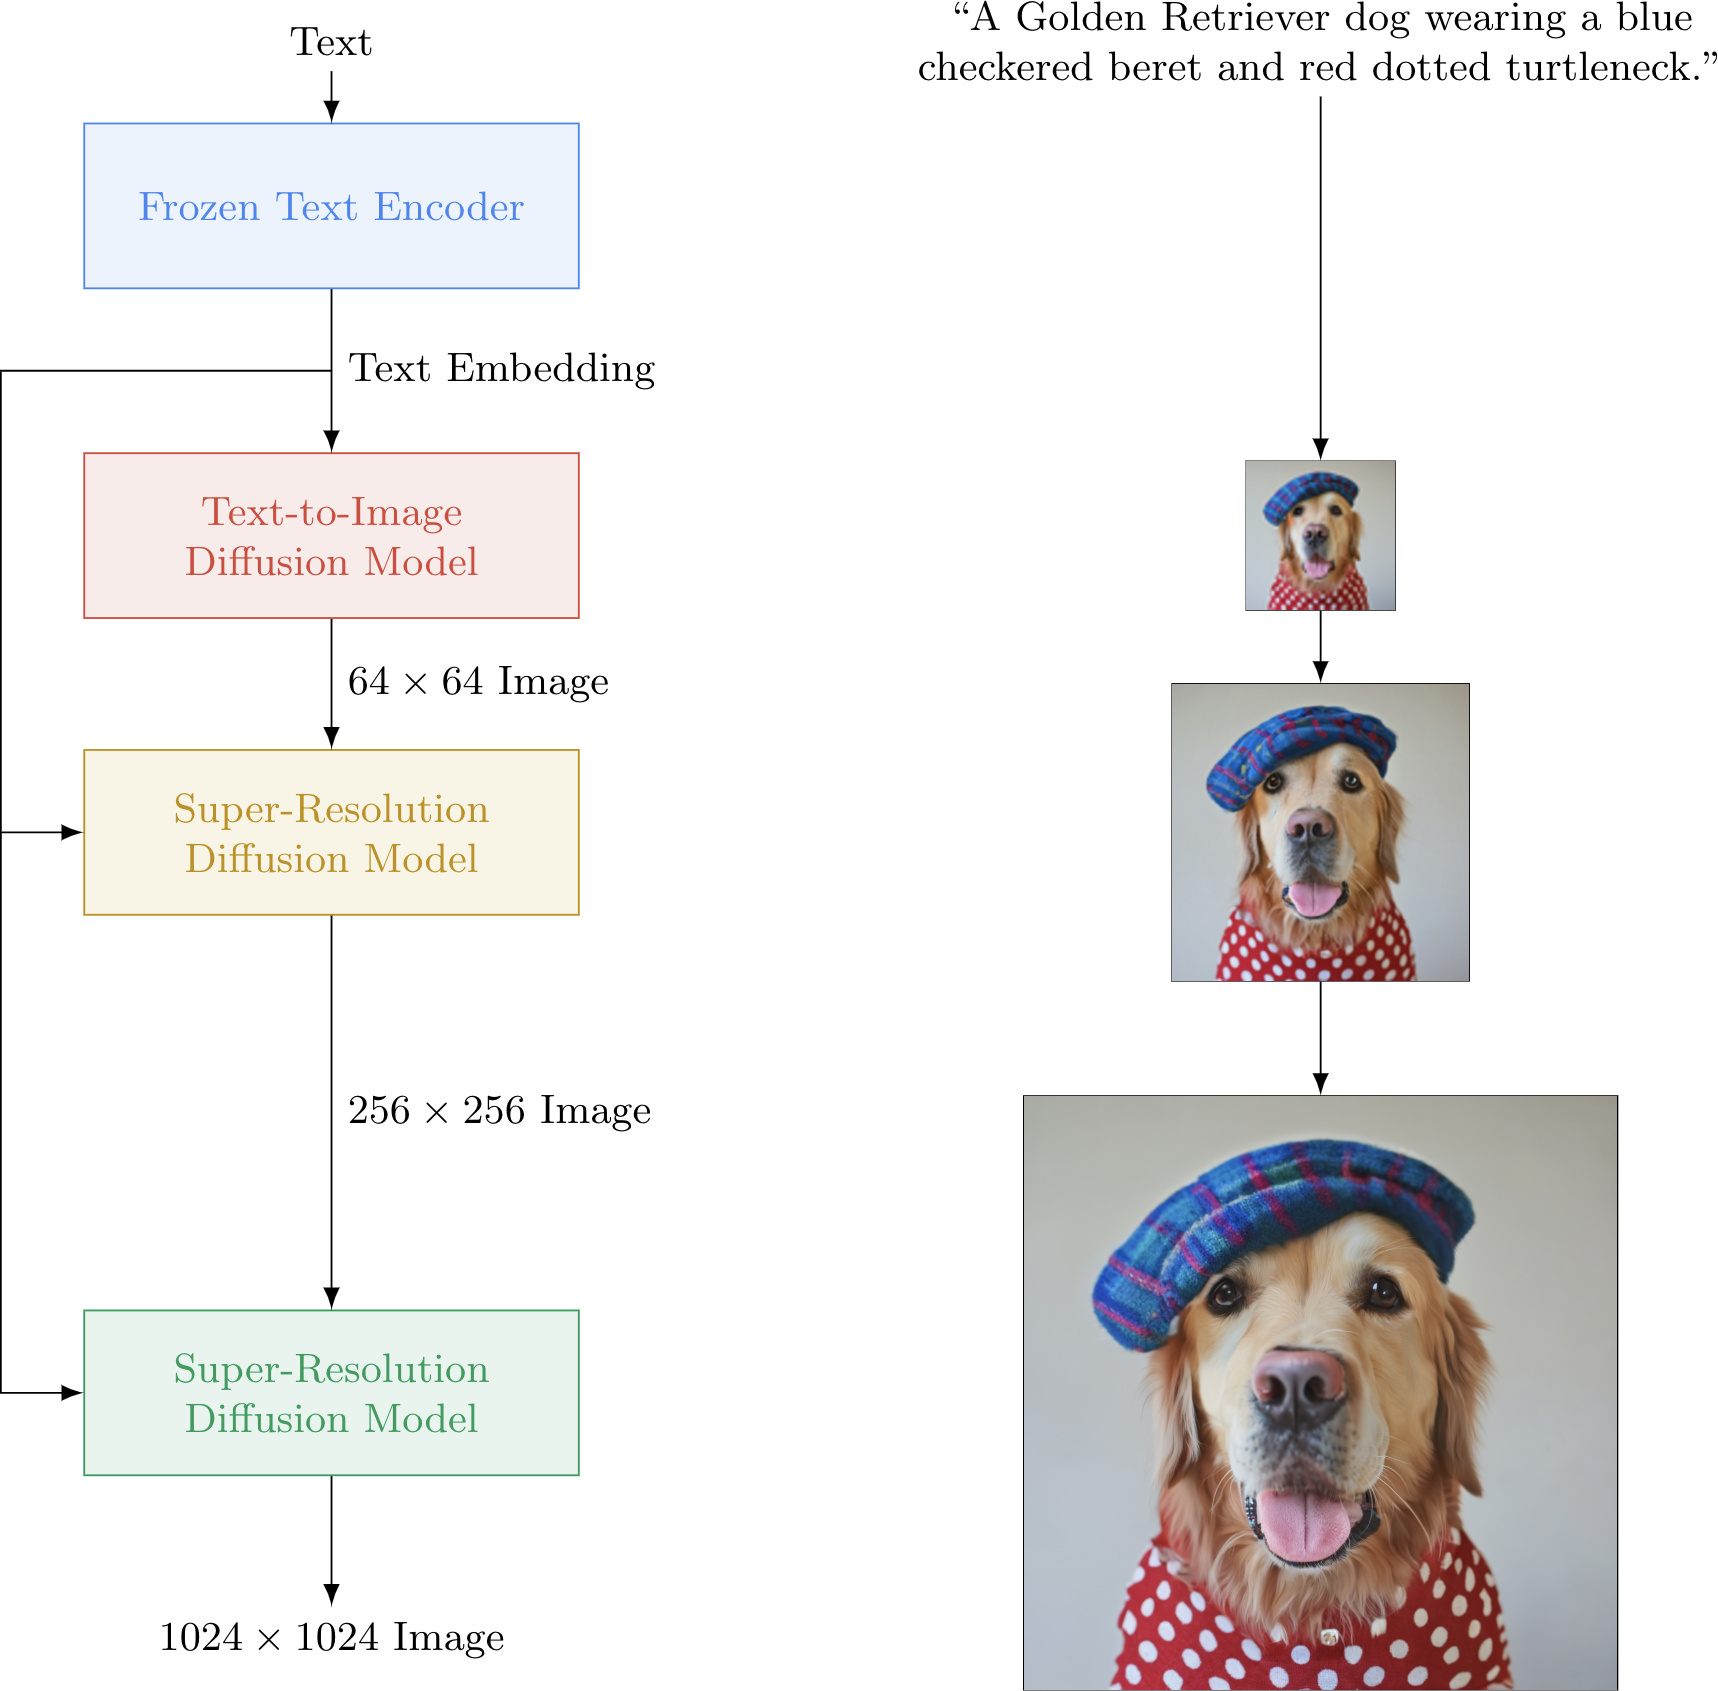
\includegraphics[width=1.0\textwidth]{text_to_image_diffusion.jpg}
    \captionof{figure}{Mô hình Khuếch tán cho việc sinh ảnh từ văn bản. Bắt đầu từ nhiễu, mô hình dần dần khử nhiễu theo sự dẫn dắt của embedding văn bản để tạo ra ảnh cuối cùng.}
    \label{fig:text_to_image_diffusion}
\end{center}

\subsubsection{Sinh Video từ Văn bản (Text-to-Video)}
Là một bước tiến tự nhiên nhưng khó hơn rất nhiều so với sinh ảnh.
\begin{itemize}
    \item \textbf{Thách thức chính:} Ngoài việc tạo ra các khung hình (frames) chất lượng cao, mô hình còn phải đảm bảo \textbf{tính nhất quán về mặt thời gian (temporal consistency)}. Các đối tượng và bối cảnh phải duy trì sự logic và liền mạch từ khung hình này sang khung hình tiếp theo.
    \item \textbf{Hướng tiếp cận:} Các mô hình tiên tiến như Sora (OpenAI) hay Lumiere (Google) mở rộng ý tưởng của mô hình khuếch tán sang không-thời gian. Chúng không xử lý từng khung hình riêng lẻ mà xử lý một loạt các khung hình hoặc toàn bộ "patch" không-thời gian cùng lúc để đảm bảo sự mượt mà và nhất quán của chuyển động và bối cảnh.
\end{itemize}

Việc làm chủ khả năng sinh đa phương thức không chỉ mở ra những ứng dụng sáng tạo mới mà còn là một bước tiến quan trọng hướng tới các hệ thống AI có khả năng tương tác và sáng tạo trong một thế giới đa dạng về phương thức như thế giới của chúng ta.

\subsection{Kiểm soát Quá trình Sinh (Controlled Generation)}
\label{ssec:controlled_generation}

Trong nhiều ứng dụng thực tế, yêu cầu không chỉ dừng lại ở việc sinh văn bản mạch lạc và tự nhiên, mà còn phải đảm bảo \textbf{tuân theo các ràng buộc} (constraints) hoặc \textbf{thuộc tính} (attributes) cụ thể. Ví dụ:
\begin{itemize}
    \item Sinh bài đánh giá sản phẩm với \textit{sentiment} tích cực.
    \item Viết tóm tắt nhưng \textbf{giữ nguyên thuật ngữ chuyên ngành}.
    \item Sinh hội thoại chatbot với \textbf{giọng điệu thân thiện}.
\end{itemize}

Đây là bài toán về việc ``\textbf{lái}'' quá trình sinh ngôn ngữ của LLM theo mong muốn của người dùng hoặc hệ thống.

\subsubsection{Các kỹ thuật kinh điển}
\label{sssec:classic_controlled_generation}

\paragraph{CTRL (Conditional Transformer Language Model)}
\begin{itemize}
    \item Ý tưởng: thêm các \textbf{mã kiểm soát (control codes)} đặc biệt vào đầu prompt để chỉ định thuộc tính mong muốn. 
    \item Ví dụ: \texttt{Reviews Rating: 5.0 The product was ...} để mô hình sinh tiếp một đánh giá tích cực.
    \item Ưu điểm: đơn giản, trực quan.
    \item Nhược điểm: đòi hỏi mô hình được \textbf{huấn luyện lại từ đầu} với dữ liệu gắn kèm mã kiểm soát; khó áp dụng cho nhiều thuộc tính phức tạp.
\end{itemize}

\paragraph{PPLM (Plug and Play Language Models)}
\begin{itemize}
    \item Ý tưởng: sử dụng một \textbf{mô hình thuộc tính nhỏ} (ví dụ: bộ phân loại cảm xúc) để hướng dẫn LLM đã đóng băng. 
    \item Cách làm: tại mỗi bước sinh, gradient từ mô hình thuộc tính sẽ \textbf{điều chỉnh trạng thái ẩn} của LLM để tăng xác suất sinh ra từ phù hợp.
    \item Ưu điểm: không cần huấn luyện lại LLM lớn; dễ áp dụng cho nhiều thuộc tính.
    \item Nhược điểm: chi phí tính toán cao do phải tính gradient trong lúc sinh; có thể làm giảm độ mạch lạc.
\end{itemize}

\paragraph{FUDGE (Future Discriminators for Generation)}
\begin{itemize}
    \item Thay vì chỉnh trực tiếp trạng thái ẩn, FUDGE huấn luyện một bộ phân loại để ước lượng \textbf{khả năng tiếp diễn thoả mãn thuộc tính}, sau đó kết hợp với xác suất sinh từ mô hình chính.
    \item Ưu điểm: linh hoạt, không cần huấn luyện lại LLM lớn.
    \item Nhược điểm: vẫn bị trade-off giữa kiểm soát và chất lượng.
\end{itemize}

\subsubsection{Các kỹ thuật dựa trên Prompt}
\label{sssec:prompt_based_controlled_generation}

Các phương pháp này thuộc nhóm \textbf{PEFT (Parameter-Efficient Fine-Tuning)} và hiện được ứng dụng rộng rãi do hiệu quả cao.

\paragraph{Prompt Tuning}
\begin{itemize}
    \item Học các \textbf{prompt mềm (soft prompts)} — tức là các vector embedding có thể học được — để hướng dẫn mô hình.
    \item Ví dụ: để điều khiển văn bản theo giọng điệu ``lịch sự'', ta học một soft prompt tương ứng và nối nó vào trước input.
    \item Ưu điểm: nhẹ, không cần tinh chỉnh toàn bộ mô hình.
    \item Nhược điểm: hiệu quả hạn chế nếu số lượng thuộc tính cần kiểm soát quá nhiều.
\end{itemize}

\paragraph{Prefix Tuning}
\begin{itemize}
    \item Ý tưởng: học các vector embedding ``tiền tố'' và \textbf{chèn vào mỗi lớp Transformer}.
    \item Nhờ vậy, prompt không chỉ ảnh hưởng ở input mà còn tác động trực tiếp lên \textbf{attention} của mọi tầng.
    \item Hiệu quả hơn Prompt Tuning trong nhiều tác vụ yêu cầu kiểm soát tinh vi.
\end{itemize}

\paragraph{LoRA (Low-Rank Adaptation) và Adapter Tuning}
\begin{itemize}
    \item LoRA chèn thêm ma trận hạng thấp vào trong trọng số attention, trong khi Adapter Tuning chèn ``mô-đun phụ'' vào giữa các lớp Transformer.
    \item Cả hai cho phép học thêm một số ít tham số để kiểm soát phong cách, giọng điệu hoặc thuộc tính sinh.
\end{itemize}

\paragraph{In-Context Control}
\begin{itemize}
    \item Không cần tinh chỉnh mô hình, chỉ cần đưa \textbf{ví dụ minh hoạ (few-shot)} vào prompt.
    \item Ví dụ: nếu muốn mô hình sinh phản hồi ngắn gọn, ta có thể thêm vào prompt vài ví dụ ``câu trả lời ngắn''.
    \item Đây là phương pháp thực tế nhất trong triển khai API, tuy nhiên không ổn định khi yêu cầu phức tạp.
\end{itemize}

\subsubsection{Các hướng mở rộng hiện đại}
\begin{itemize}
    \item \textbf{RLHF (Reinforcement Learning from Human Feedback)}: dùng con người để đánh giá và tinh chỉnh chính sách sinh, giúp mô hình tuân theo các chuẩn mực xã hội.
    \item \textbf{Direct Preference Optimization (DPO)}: thay thế RLHF truyền thống bằng tối ưu trực tiếp trên dữ liệu so sánh, đơn giản hơn.
    \item \textbf{Control bằng ràng buộc hình thức}: ví dụ đảm bảo output phải là JSON hợp lệ, hoặc đảm bảo không vi phạm regex.
    \item \textbf{Multi-attribute control}: điều khiển đồng thời nhiều thuộc tính (ví dụ: văn bản vừa ``tích cực'' vừa ``ngắn gọn'').
\end{itemize}

\subsection{Sinh Nhận biết Cấu trúc (Structure-aware Generation)}
\label{ssec:structure_aware_generation}

Một thách thức lớn khác là sinh ngôn ngữ tự nhiên từ dữ liệu có cấu trúc (\textit{structured data}) như \textbf{bảng}, \textbf{cơ sở dữ liệu}, hoặc \textbf{đồ thị tri thức}. Đây là nền tảng cho nhiều ứng dụng: báo cáo tự động, sinh mô tả sản phẩm, hoặc trợ lý ảo truy vấn dữ liệu.

\subsubsection{Sinh Văn bản từ Bảng (Table-to-text)}
\begin{itemize}
    \item \textbf{Bài toán:} Cho một bảng dữ liệu, sinh ra đoạn văn mô tả hoặc tóm tắt thông tin.
    \item \textbf{Hướng tiếp cận:}
    \begin{enumerate}
        \item \textbf{Tuyến tính hoá (linearization)}: biến bảng thành chuỗi 1D với các token đặc biệt cho hàng/cột/ô, rồi dùng Seq2Seq (T5, BART).
        \item \textbf{Schema-guided generation}: tận dụng nhãn cột/hàng để hướng dẫn mô hình.
        \item \textbf{Pretraining đặc thù}: ví dụ TAPAS (Google) huấn luyện trực tiếp trên bảng + câu hỏi.
    \end{enumerate}
\end{itemize}

\subsubsection{Sinh Văn bản từ Đồ thị (Graph-to-text)}
\begin{itemize}
    \item \textbf{Bài toán:} Cho một đồ thị tri thức (Knowledge Graph), sinh ra mô tả bằng ngôn ngữ tự nhiên.
    \item \textbf{Hướng tiếp cận:}
    \begin{enumerate}
        \item \textbf{Mạng nơ-ron đồ thị (GNN)} để mã hoá cấu trúc quan hệ thành embedding.
        \item Transformer \textbf{attend} lên embedding này để sinh chuỗi văn bản.
        \item Một số mô hình tiêu biểu: \textit{GraphWriter}, \textit{KG-to-Text}.
    \end{enumerate}
\end{itemize}

\subsubsection{Sinh Văn bản từ CSDL (Data-to-text)}
\begin{itemize}
    \item \textbf{Ví dụ:} Sinh báo cáo tài chính tự động từ số liệu.
    \item \textbf{Cách làm:} Tương tự table-to-text nhưng bổ sung thêm cơ chế \textbf{content planning} để quyết định thông tin nào cần nhắc đến trước.
\end{itemize}
